\section{\isklearn pipeline composition per dataset}

Pipeline structures selected by \irace for each dataset are given as sunburst plots in Figure~\ref{fig:dataset_composition}. First, a different predictor is mostly selected for each of the CV problems: for CIFAR-10 6 out of 10 pipelines used LR, followed by SVM twice, and once each for kNN and MLP; for FMNIST, SVM was predominant, chosen in seven runs, with LR chosen twice and MLP once; and for SVHN, it was kNN, also chosen 7 times, with the remaining three equally divided between MLP, AB, and DT. In addition, preprocessing is increasingly adopted in these datasets, in this same order: while only 3 pipelines used any kind of preprocessing for CIFAR-10, only one did not for SVHN.

Concerning TS problems, LR is frequently selected (6 times) for the Boston dataset, followed by SVM (twice) and MLP (once), whereas for the Natal dataset SVM, LR, and MLP are uniformly distributed. Preprocessing patterns for TS problems are little affected by the particularities of each dataset, with \texttt{\small Selection} being universally adopted and additionally \texttt{\small Extraction} in some cases. Finally, as already discussed in this paper, LR is predominant in the pipelines for the NLP datasets. Furthermore, preprocessing is rarely used here, with only Reuters adopting any kind of preprocessing more than once, mostly through \texttt{\small Extraction}.

\begin{figure*}
    \centering
    
  	\begin{subfigure}[t]{0.3\textwidth}
    \centering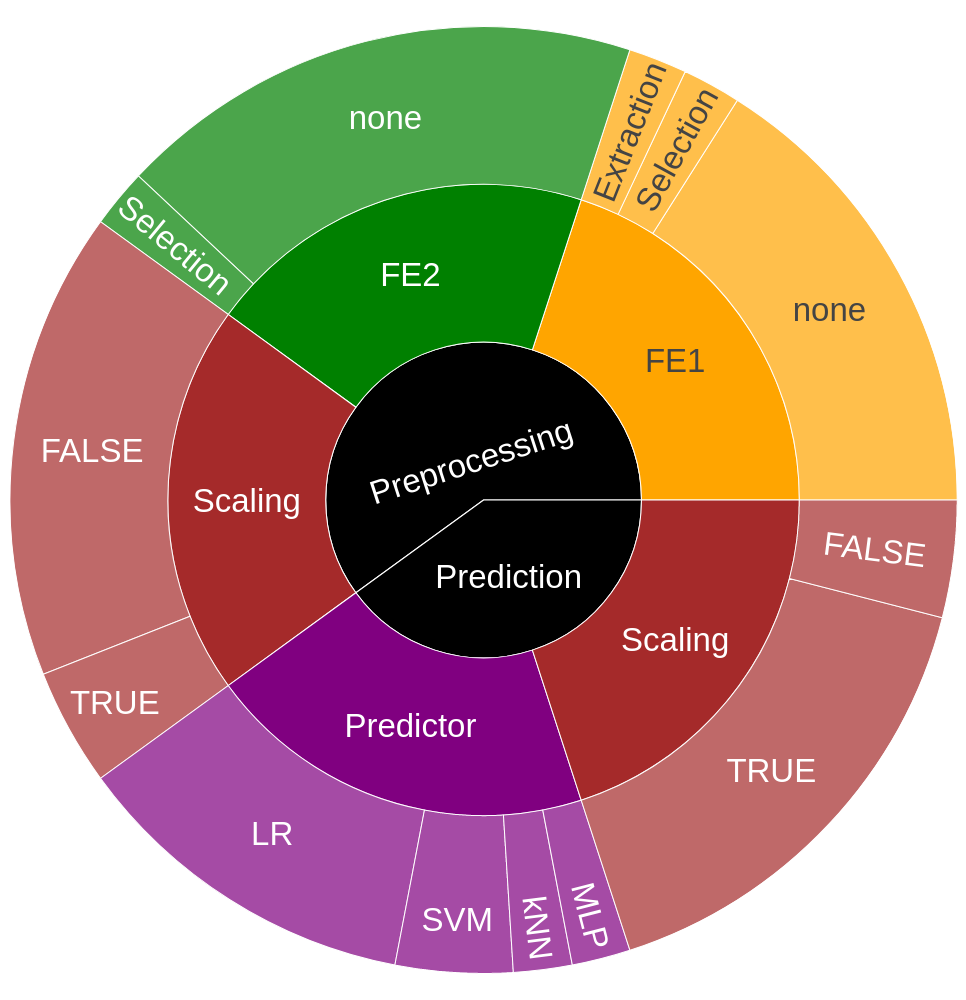
\includegraphics[width=\textwidth]{img/sunburst/cifar10.png}
    \caption{CIFAR-10}
  	\end{subfigure}
  	\begin{subfigure}[t]{0.3\textwidth}
    \centering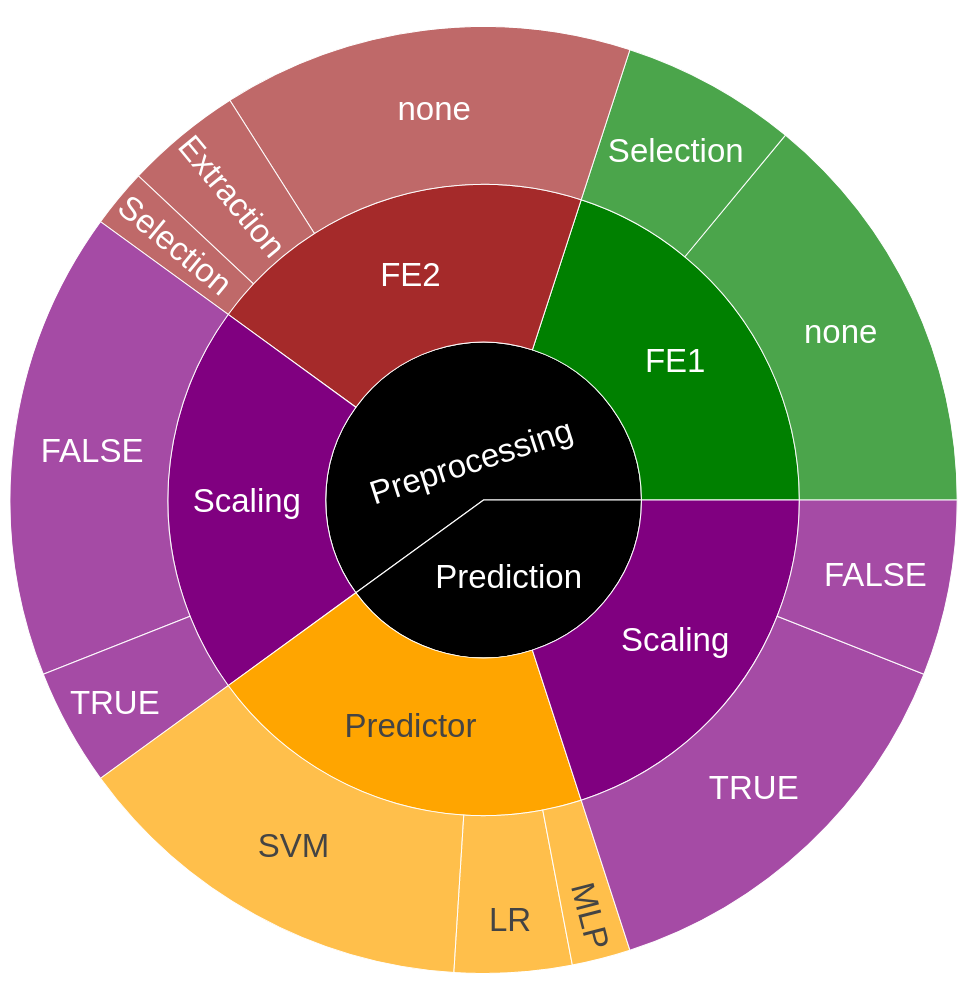
\includegraphics[width=\textwidth]{img/sunburst/fmnist.png}
    \caption{FMNIST}
  	\end{subfigure}
	\begin{subfigure}[t]{0.3\textwidth}
    \centering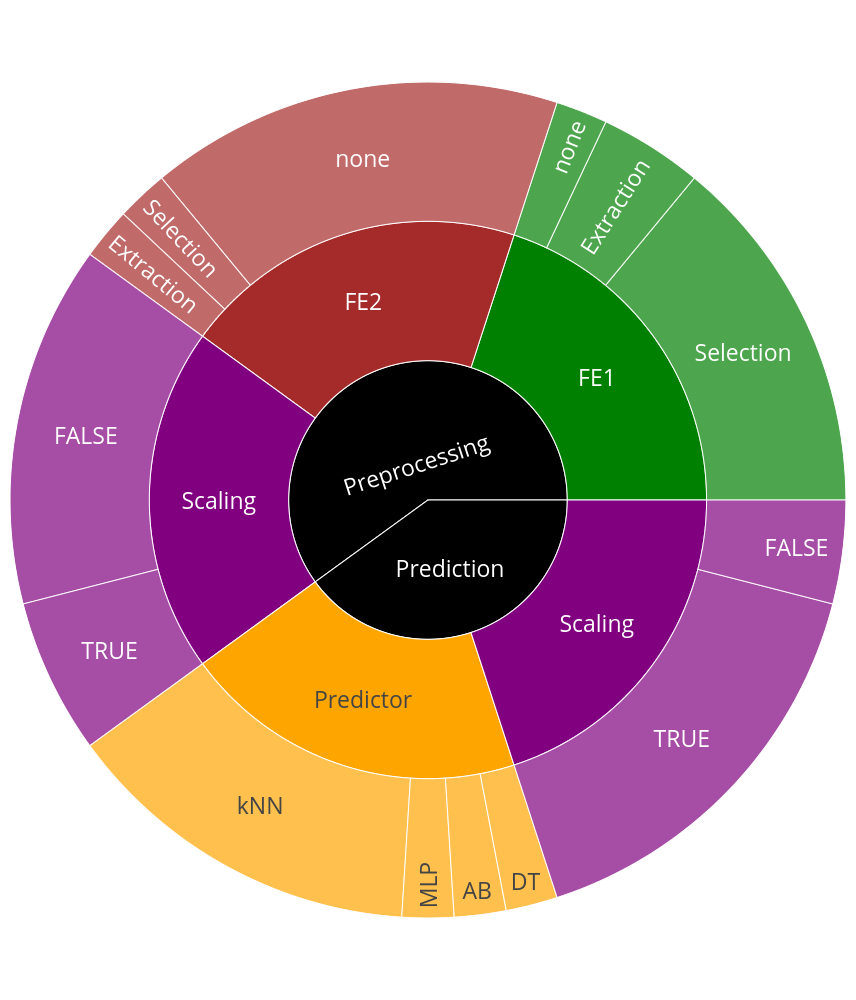
\includegraphics[width=\textwidth]{img/sunburst/svhn.png}
    \caption{SVHN}
  	\end{subfigure}

  	\begin{subfigure}[t]{0.3\textwidth}
    \centering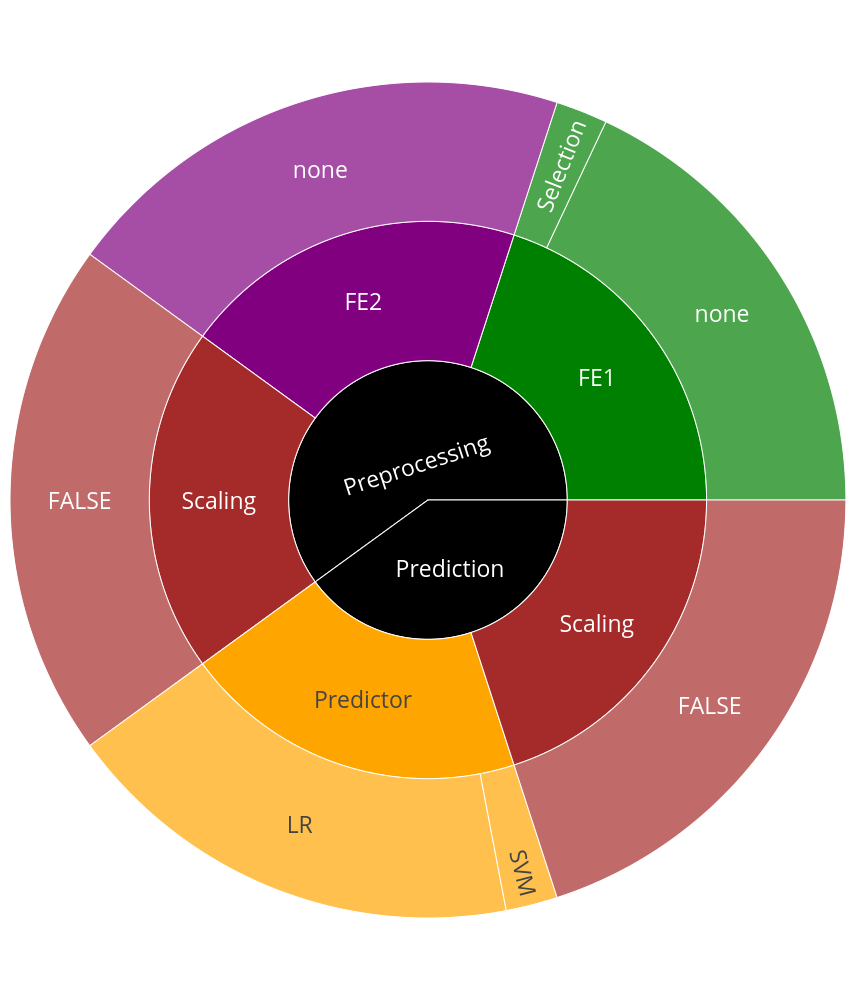
\includegraphics[width=\textwidth]{img/sunburst/lmrd.png}
    \caption{LMRD}
  	\end{subfigure}
  	\begin{subfigure}[t]{0.3\textwidth}
    \centering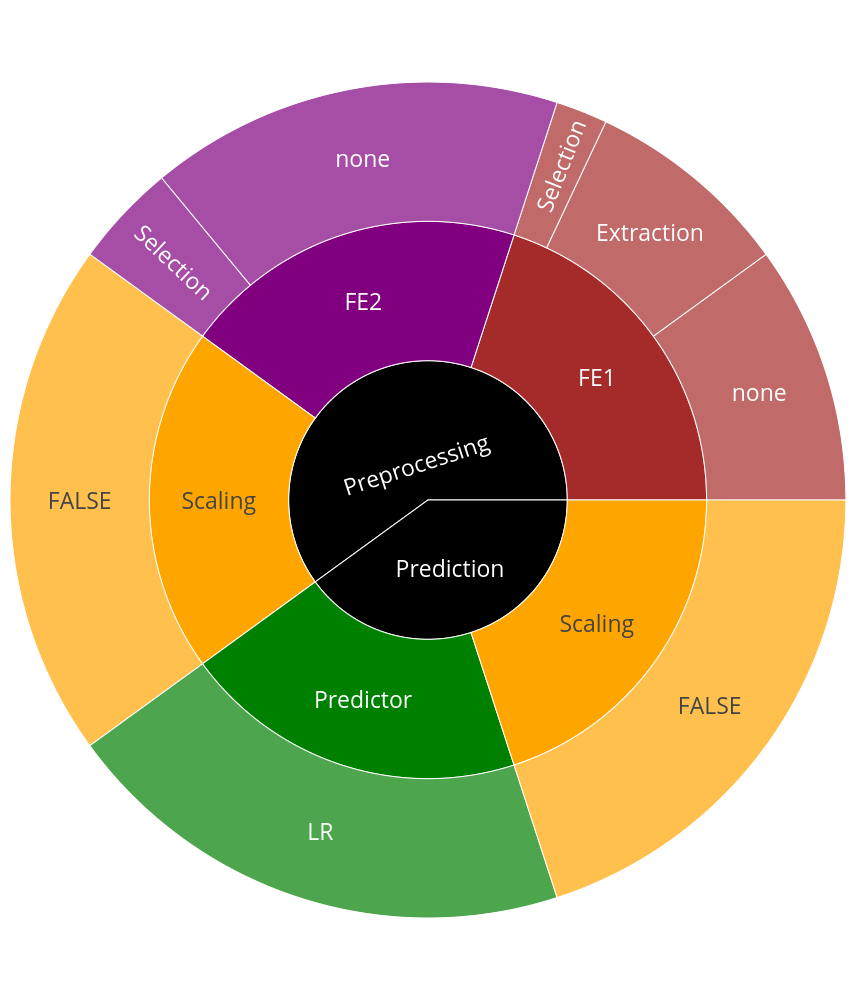
\includegraphics[width=\textwidth]{img/sunburst/reuters.png}
    \caption{Reuters}
  	\end{subfigure}
	\begin{subfigure}[t]{0.3\textwidth}
    \centering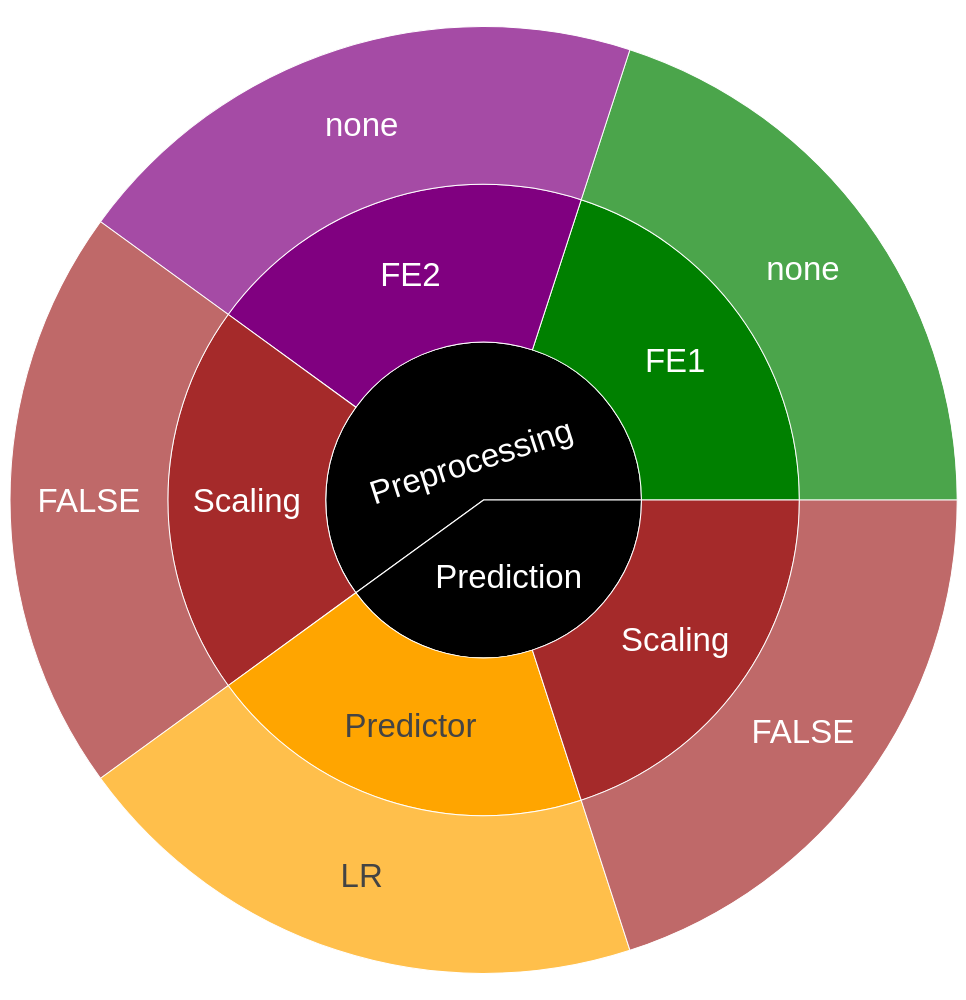
\includegraphics[width=\textwidth]{img/sunburst/agnews.png}
    \caption{AGNews}
  	\end{subfigure}

  	\begin{subfigure}[t]{0.3\textwidth}
    \centering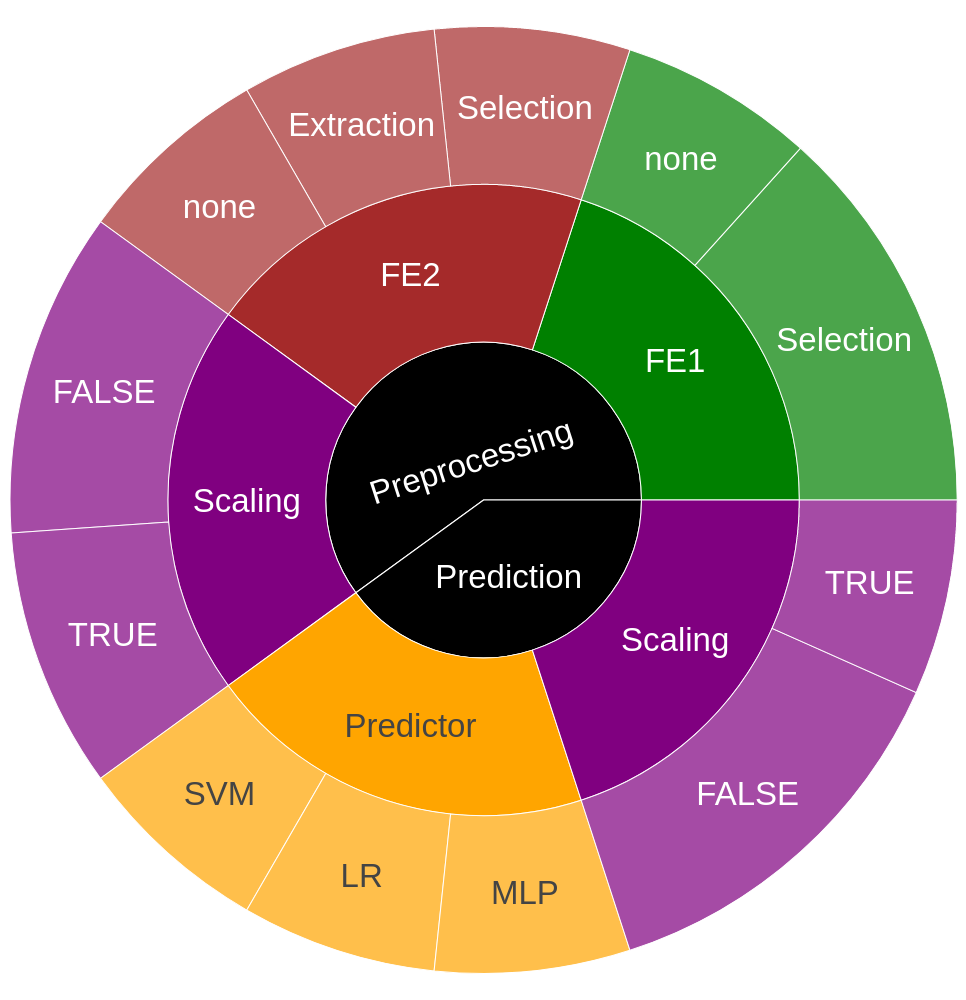
\includegraphics[width=\textwidth]{img/sunburst/natal.png}
    \caption{Natal}
  	\end{subfigure}
	\begin{subfigure}[t]{0.3\textwidth}
    \centering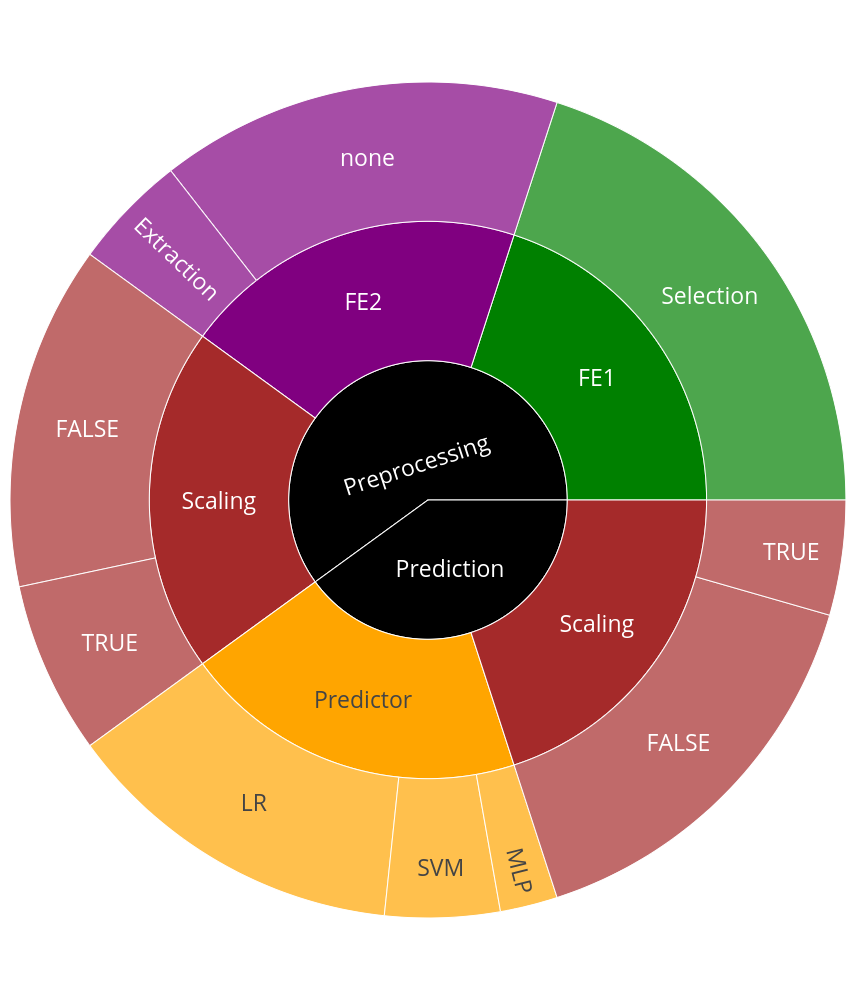
\includegraphics[width=\textwidth]{img/sunburst/boston.png}
    \caption{Boston}
  	\end{subfigure}

    \caption{Pipeline composition for each dataset.}
    \label{fig:dataset_composition}
\end{figure*}

\section{Variance analysis for regular setup}
We provide variance analysis for the results shown in Table~\ref{tb:results} through boxplots, given in Figure~\ref{fig:vanilla-boxplots}.

\begin{figure*}
    \centering
    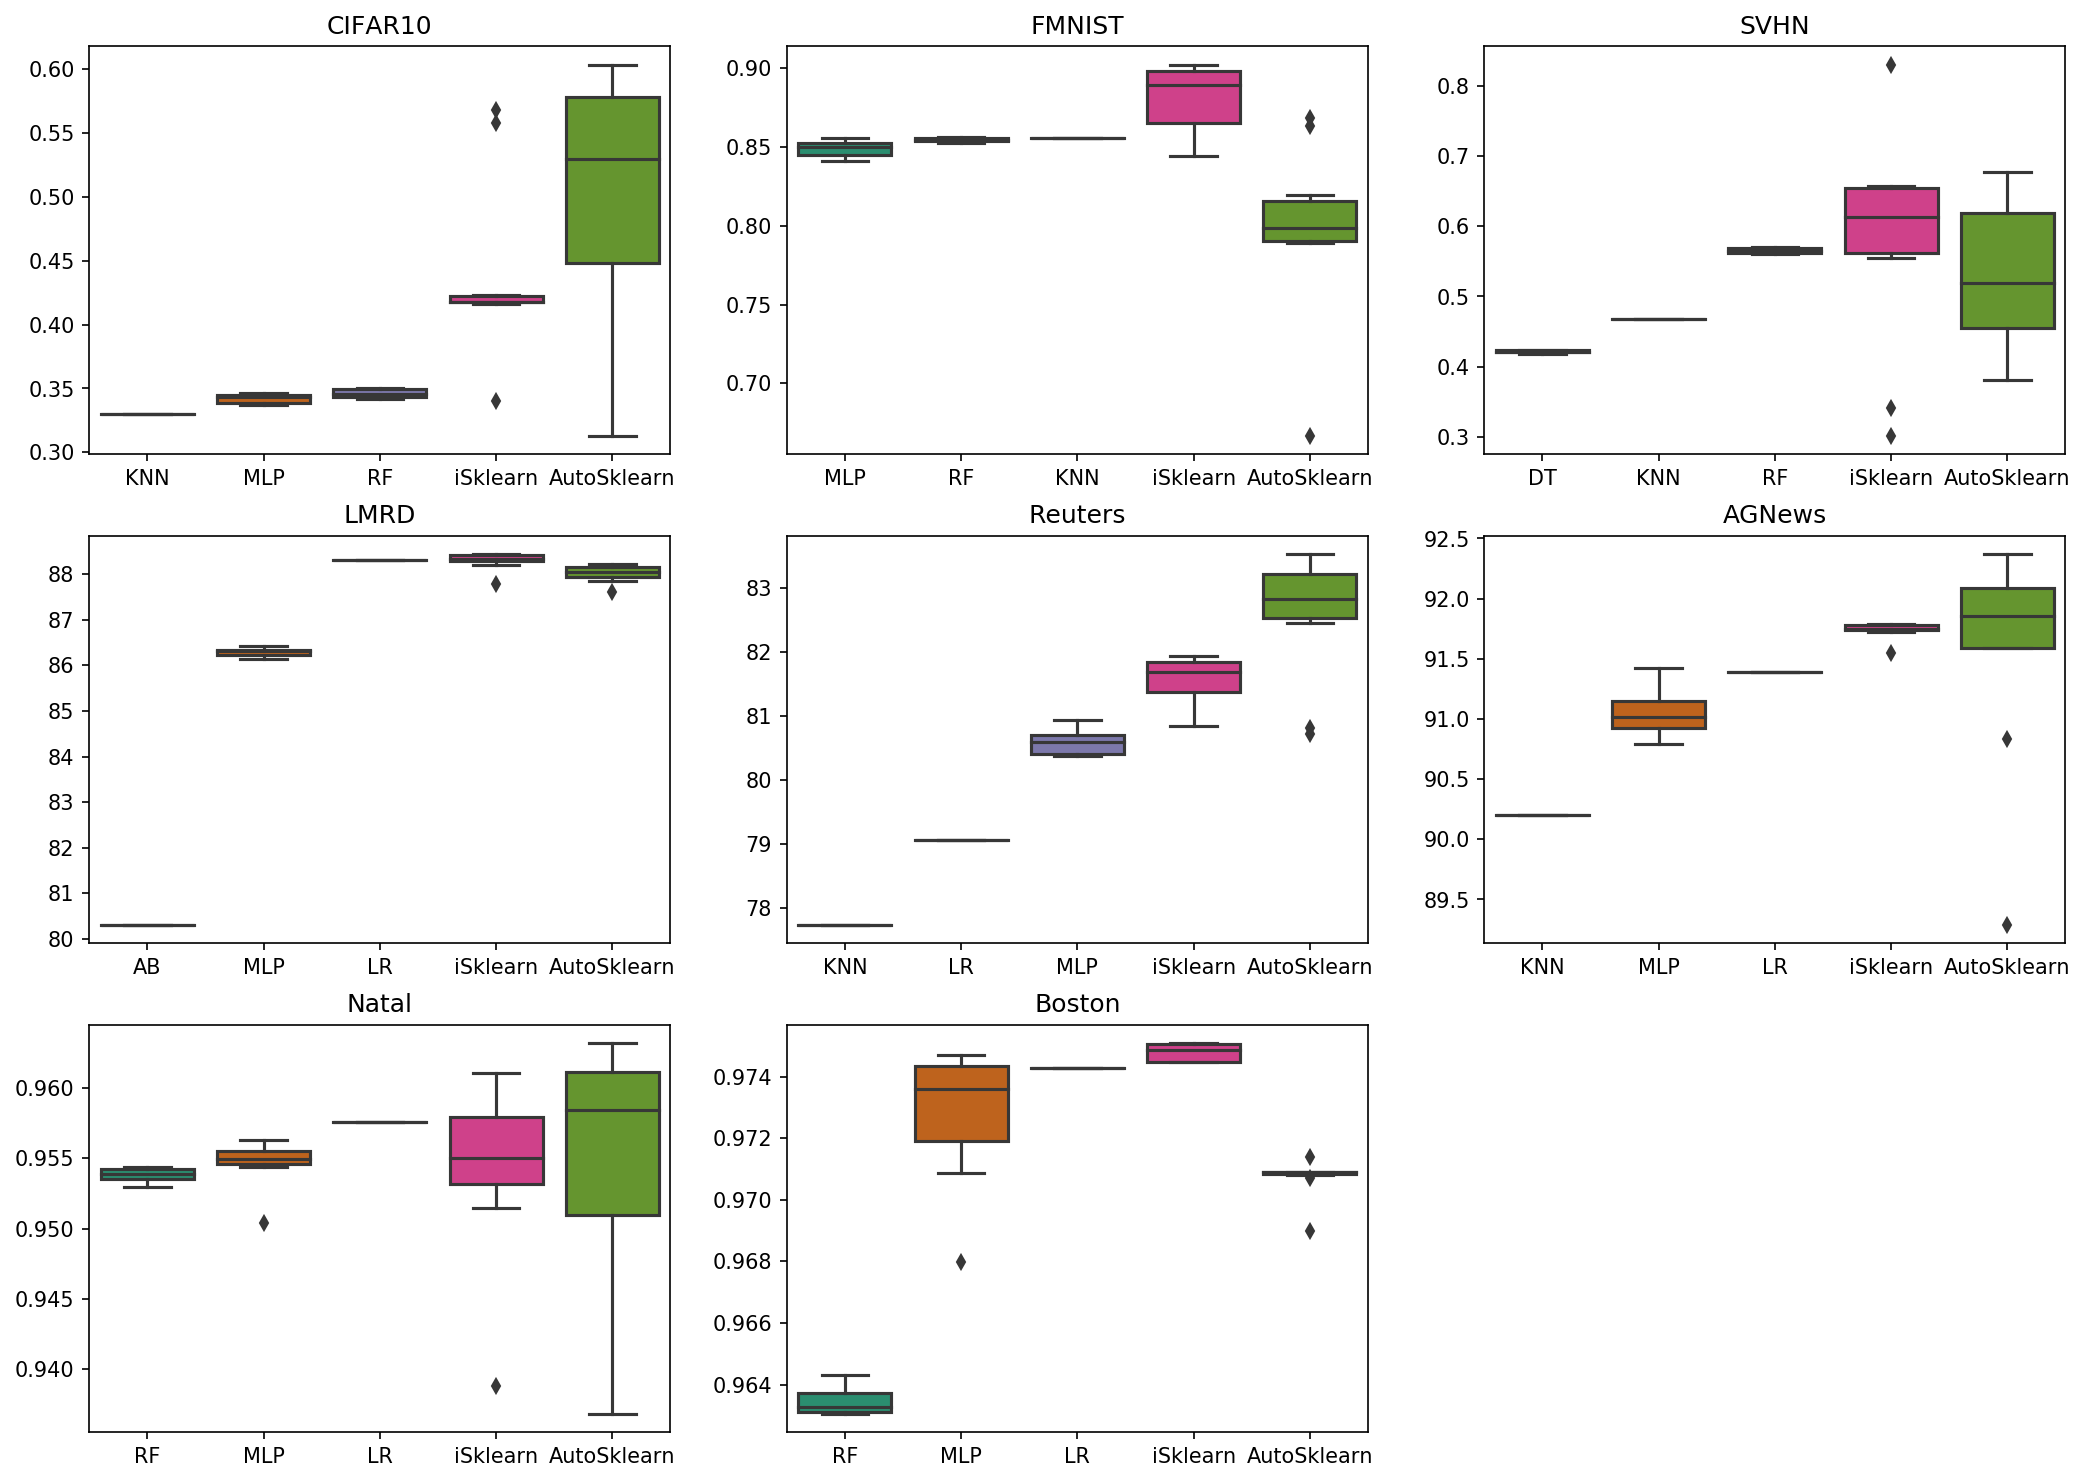
\includegraphics[width=\textwidth]{img/vanilla-boxplots.png}
    \caption{Accuracy~(\%) and $R^2$ score comparison between pipelines configured by \isklearn, ensembles produced by \autosklearn, as well as the three best-performing default models for each dataset.}
    \label{fig:vanilla-boxplots}
\end{figure*}